\documentclass[10pt]{article}
\usepackage[margin=0.75in]{geometry}
\usepackage{graphicx}
\usepackage{amsmath}
\usepackage{enumitem}
\usepackage[font=footnotesize,it,skip=2pt]{caption}
\usepackage{float}
\usepackage{titlesec}
\usepackage[colorlinks=true, linkcolor=black, citecolor=black, urlcolor=magenta]{hyperref}

\titleformat{\section}
  {\normalfont\fontsize{12}{12}\bfseries} % 12pt font with 15pt spacing
  {\thesection}{1em}{}

\titleformat{\subsection}
  {\normalfont\fontsize{11}{11}\bfseries}
  {\thesubsection}{1em}{}

\titleformat{\subsubsection}
  {\normalfont\fontsize{10}{10}\bfseries}
  {\thesubsubsection}{1em}{}


\begin{document}

\begin{titlepage}
    \centering
    \vspace*{5cm}
    {\LARGE Hybrid Quantum-Classical Neural Networks\\ for Stock Price Forecasting\par}
    \vspace{3cm}
    {\Large Nathaniel James Pacey\par}
    \vspace{0.5cm}
    {\large \textit{Terra Quantum}\par}
    \vfill
    {\large \today\par}
\end{titlepage}

\section*{1. Introduction}

Stock market data presents a challenging and realistic benchmark for evaluating machine learning models due to its inherent complexity and dependence on a multitude of socio-economic factors ~\cite{madisson2019stockrnn, chen2023options}. Modeling and preprocessing strategies were adapted from my bachelor's thesis on RNN-based forecasting of American-style stock options.



\section*{2. Methodology}
\subsection*{2.1 Data Source and Preprocessing}

Stock prices are unbounded and influenced by factors such as macroeconomics, sentiment, volatility, and corporate events. Events like stock splits alter share prices without affecting value, potentially misleading models if not handled correctly~\cite{jahan2018stock, chen2023options}. Understanding such structural behavior is essential for reliable forecasting. This work uses daily closing prices for \textbf{AAPL}, \textbf{MSFT}, and \textbf{GOOGL} from \textbf{January 1, 2015} to \textbf{December 31, 2024}, obtained via the \texttt{yfinance} API. Missing values were forward-filled to maintain continuity, and prices were normalized per ticker using \textbf{Min-Max scaling} to the range \textbf{[0, 1]}~\cite{lesuisse2022americanoptions}. To structure the data for forecasting, a \textbf{sliding window} of \textbf{20} time steps was applied, with each sequence mapped to its next price value. This approach preserved short-term dependencies and momentum patterns~\cite{fischer2018lstm}. Data was split into training and testing sets using a time-respecting \textbf{80/20} ratio, ensuring no future leakage~\cite{fischer2018lstm}. Sequences from all tickers were then combined to improve diversity and model generalization across financial instruments.

\subsection*{2.3 Model Architecture}

Given their strong performance in financial forecasting, recurrent neural networks (RNNs) were chosen as the core machine learning unit~\cite{madisson2019stockrnn, jahan2018stock}. To enable flexible experimentation and optimization, the model was designed as a fully modular framework inspired by Terra’s QAI Hub. Users can, select activation functions, adjust skip connections, apply regularization methods such as dropout and layer normalization, change the learning rate and optionally insert a quantum layer. Both the model architecture and quantum circuit are automatically visualized from configuration settings to enable rapid testing and comparison, with the final hybrid and classical models shown in Appendix~\ref{appendix:model-architecture}.


The classical processing pipeline is implemented in \texttt{PyTorch}. It begins with a user-defined sequence of recurrent layers, which may include single or mixed combinations of LSTM, GRU, and RNN units. The first recurrent block uses a configurable number of layers, while subsequent blocks default to a single layer. These layers process inputs of shape \texttt{(batch\_size, sequence\_length, 1)}, extracting temporal features from which the final hidden state is retained. This hidden state is then projected via a dense layer to match the number of qubits, forming the input to the optional quantum layer ~\cite{hochreiter1997lstm, kostadinov2017gru}.

If the quantum layer is enabled, the projected features are passed through a variational quantum circuit (built using PennyLane’s \texttt{QNode} interface, as shown in Figure~\ref{fig:final quantum circuit}~\cite{schuld2021machine}), where each feature is encoded via an RY gate~\cite{mitarai2018quantum}. Across a configurable number of variational layers (\texttt{q\_depth}), each qubit undergoes a parameterized rotation: either \texttt{RY} (1 parameter), \texttt{RX + RZ} (2 parameters), or \texttt{Rot} (3 parameters). After each layer, qubits are entangled via a ring of \texttt{CNOT} gates to create a circular topology~\cite{benedetti2019parameterized}. The output is obtained by measuring the expectation value of \texttt{PauliZ} on each qubit, producing a real-valued vector.

\begin{figure}[h!]
    \centering
    \vspace{-0.8em}
    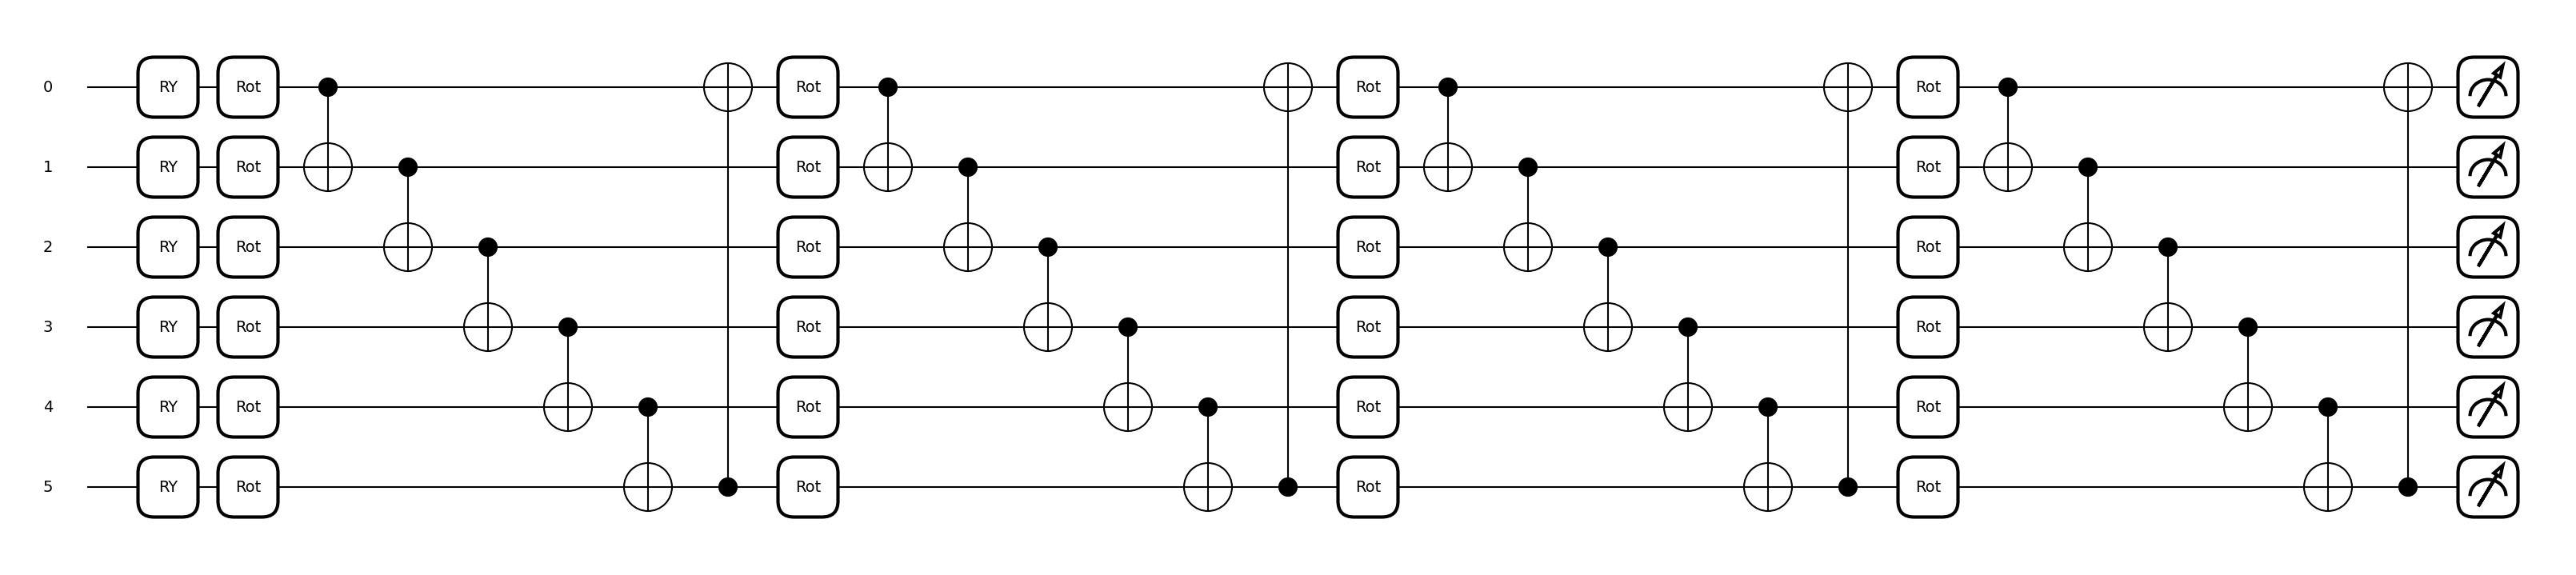
\includegraphics[trim=0.0cm 0cm 0cm 0cm,clip,width=0.7\paperwidth]{images/quantum circuit 6 4 3.png}
    \caption{Optimal quantum circuit with \texttt{n\_qubits=6}, \texttt{q\_depth=4}, and \texttt{Rot} gates.}
    \label{fig:final quantum circuit}
    \vspace{-0.6em}
\end{figure}

Post-quantum processing optionally applies non-linear activation functions (e.g., \texttt{Tanh}, \texttt{Sigmoid}) and regularization (dropout, layer normalization). The quantum output and pre-quantum classical features are merged either by concatenation or addition, depending on the \texttt{skip\_connection} setting. The merged features are then passed through a final dense layer to generate the scalar prediction, optionally followed by an output activation function.


\subsection*{2.4 Training Strategy}

The model was trained using the \textbf{mean squared error (MSE)} loss function and the \textbf{Adam} optimizer with a \textbf{learning rate of 0.001}~\cite{goodfellow2016deep}. To prevent overfitting, \textbf{early stopping} was applied with a patience window of 2–4 epochs depending on the experiment. During training, both \textbf{training loss} and \textbf{validation loss} were computed at every epoch. If no improvement in validation loss was observed within the specified patience, training was halted early. A training budget of \textbf{10 epochs} was used during experimentation, while \textbf{40 epochs} were allocated for final model evaluations. The best-performing model checkpoint (based on validation loss) was saved and later reloaded for testing. Model performance was evaluated using \textbf{MAE} (mean absolute error), \textbf{RMSE} (root mean squared error), and the \textbf{average percentage error} between predicted and true price values. Loss curves were also plotted to visualize convergence behavior and training dynamics ~\cite{goodfellow2016deep}.



\section*{2. Experimental Findings}

Model design choices were guided by empirical results rather than assumptions. A series of structured experiments were conducted to evaluate different configurations of recurrent units, layer depths, dropout rates, activation functions, and quantum circuit parameters such as qubit count, depth, and rotation types.

\subsection*{2.1 Quantum Layer Optimization}

A grid search was performed over key quantum circuit parameters, \texttt{n\_qubits} from 2 to 6, \texttt{q\_depth} from 1 to 7, and \texttt{n\_rot\_params} from 1 to 3, to evaluate their influence on forecasting performance. This included all combinations of gate complexity and circuit depth, with results assessed using MAE and average percentage error as shown in Figure~\ref{fig:quantum analysis}.

\begin{figure}[H]
    \centering
    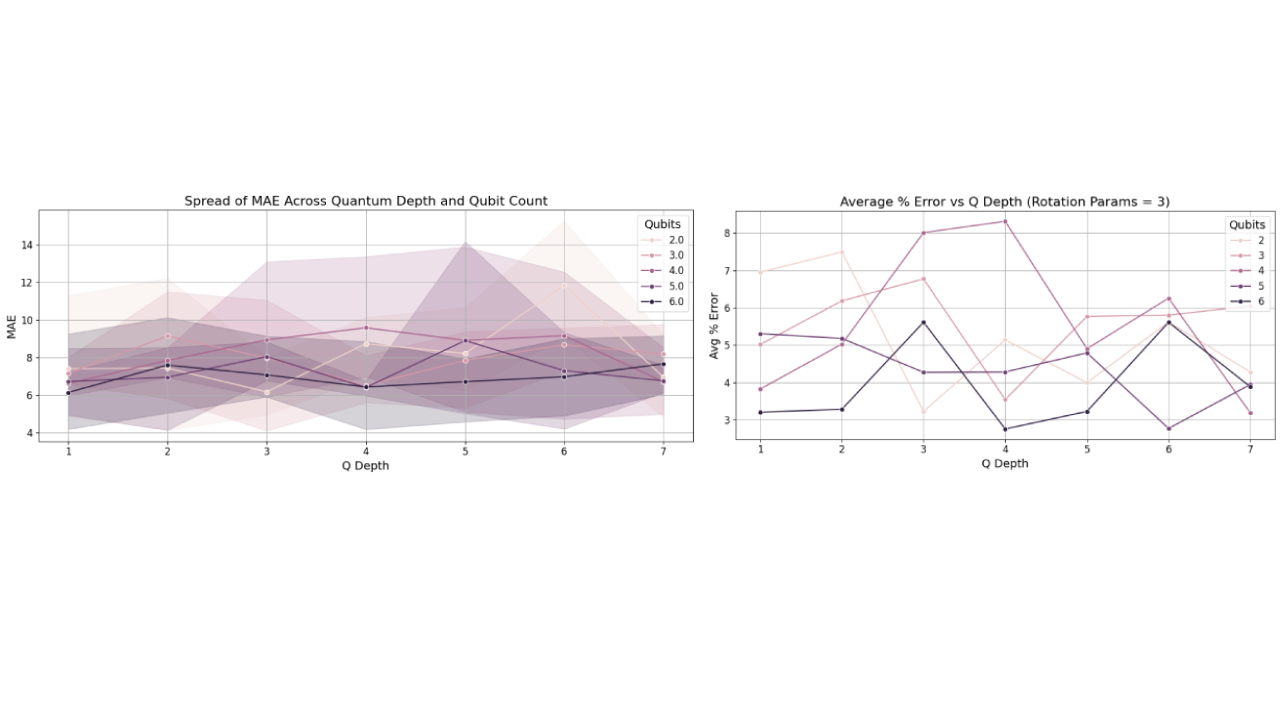
\includegraphics[trim=0cm 8cm 0cm 6.5cm,clip,width=0.8\paperwidth]{images/quantum analysis.png}
    \caption{MAE and average error across qubit counts and depths for different gate rotation types.}
    \label{fig:quantum analysis}
\end{figure}

To ensure that the quantum circuit could effectively capture the complexity of the input data, a more detailed analysis was conducted to identify when full rotation gates consistently outperformed simpler alternatives. This analysis revealed that the full rotation configuration becomes advantageous when using more than four qubits and circuit depths of at least four as seen in Appendix~\ref{appendix:rotational-sweep}. Based on these findings, the final quantum setup was selected as \texttt{n\_qubits = 6}, \texttt{q\_depth = 4}, and \texttt{n\_rot\_params = 3}.



\subsection*{2.5 Classical Architecture Optimization}
Another challenge was optimizing the classical components of the hybrid model, as training with the quantum layer is time-consuming. To enable faster experimentation, classical components were first optimized using a classical-only model with limited epochs. Modular Python scripts were developed to perform parameter sweeps, varying one parameter at a time while holding others constant~\cite{madisson2019stockrnn, kalita2023rnn, saeed2023rnnmath}. After each sweep, the best configuration was selected based on MAE, RMSE, and average percent error, and carried forward into subsequent sweeps. Coarse-grained sweeps were followed by fine-grained searches to further refine the parameter set. Parameters tested, sweep ranges, and optimal configurations are summarized in Table~\ref{tab:classical-sweep-summary}.

\begin{table}[H]
\centering
\scriptsize  % Smaller font than \small
\setlength{\tabcolsep}{4pt}  % Reduce column padding
\renewcommand{\arraystretch}{1.1}  % Adjust row height
\begin{tabular}{|l|l|l|}
\hline
\textbf{Parameter} & \textbf{Sweep Range} & \textbf{Best Result(s)} \\ \hline
Hidden Size & \{8, 16, 32, 64\} & 32 \\ \hline
Dropout Rate & \{0.0 - 0.7\} & 0.16 / None \\ \hline
Recurrent Layers & \{1–8\} & 4 \\ \hline
Recurrent Units & LSTM, GRU, RNN, combinations & GRU \\ \hline
Input / Output Activations & None, ReLU, Tanh, Sigmoid & Tanh / None \\ \hline
Skip Connection & concat, add & add \\ \hline
\end{tabular}
\caption{\scriptsize Summary of classical architecture sweeps and selected best-performing configurations.}
\label{tab:classical-sweep-summary}
\end{table}


The final hybrid quantum and classical model configuration can be seen in Figure~\ref {fig:classical-vs-quantum} and is: \texttt{GRU} with \texttt{4 layers}, \texttt{hidden size = 32}, \texttt{add skip connection}, \texttt{Tanh} post-quantum activation, and no output activation or dropout rate.



\section*{3. Results and Comparison}

To assess model performance, both training and validation losses were tracked across epochs. The final hybrid models were trained for \textbf{40 epochs}, as shown in Figure~\ref{fig:hybrid loss-curves}. The best-performing model achieved a \textbf{training loss of 0.000083} and a \textbf{validation loss of 0.000346}.


\begin{figure}[H]
    \centering
    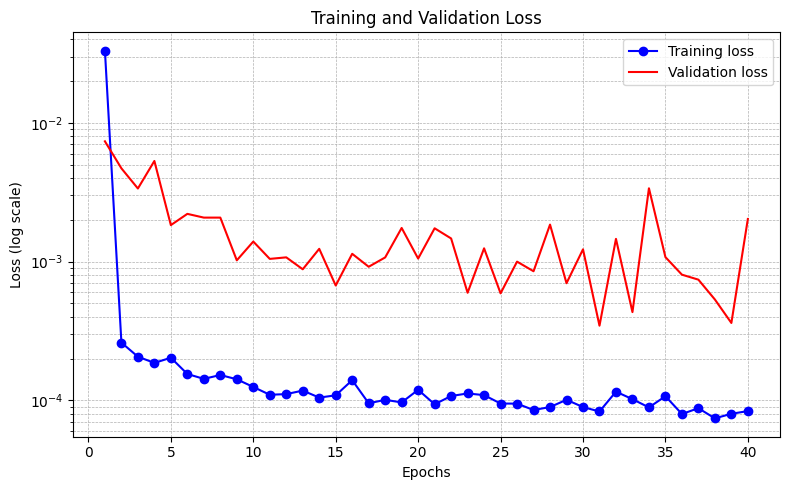
\includegraphics[trim=0cm 0cm 0cm 0.75cm,clip,width=0.6\linewidth]{images/training and validation loss GRU quantum layers.png}
    \caption{Training and validation losses over 40 epochs for the final Hybrid Quantum model.}
    \label{fig:hybrid loss-curves}
\end{figure}

While the training loss consistently decreased, the higher validation loss indicates overfitting, which is common when model capacity is high relative to data size. Reducing the number of recurrent layers or simplifying the quantum circuit may help improve generalization. However, the pattern may also reflect the \textit{double descent} phenomenon, where validation loss initially worsens before improving as model complexity increases~\cite{belkin2019reconciling}. Further investigation is needed to explore both possibilities and identify the optimal model depth, circuit design, and training duration.

To further evaluate the hybrid model's predictive performance, the following metrics were computed on the test set: \textbf{Test MAE = 2.5660}, \textbf{Test RMSE = 3.1719}, and an \textbf{Average Absolute Percentage Error of 1.77\%}. Additionally, the distribution of prediction errors was analyzed, as shown in Figure~\ref{fig:hybrid error hists}.

\begin{figure}[H]
    \centering
    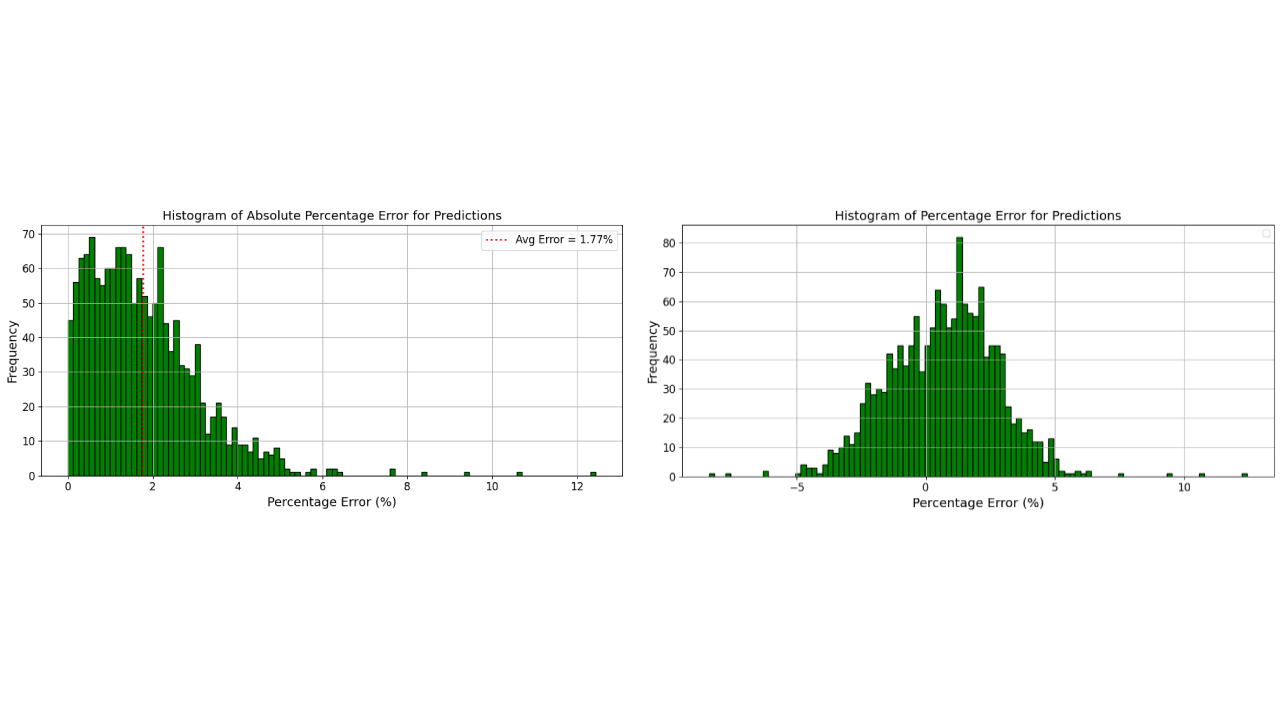
\includegraphics[trim=0cm 7cm 0cm 7.3cm,clip,width=1\linewidth]{images/hybrid prediction errors hists.png}
    \caption{Distribution of prediction errors (percentage) for the hybrid model on test data.}
    \label{fig:hybrid error hists}
\end{figure}

The histogram reveals that most prediction errors fall within 0–2\% absolute error, with the distribution centered near 0\%. This near-Gaussian error distribution around zero suggests that the hybrid model achieved a high level of accuracy and produced unbiased predictions on the test data. The predicted results for a sample stock (\textbf{GOOGL}) are visualized against the true price values in Figure~\ref{fig:Google predictions hybrid}.

\begin{figure}[H]
    \centering
    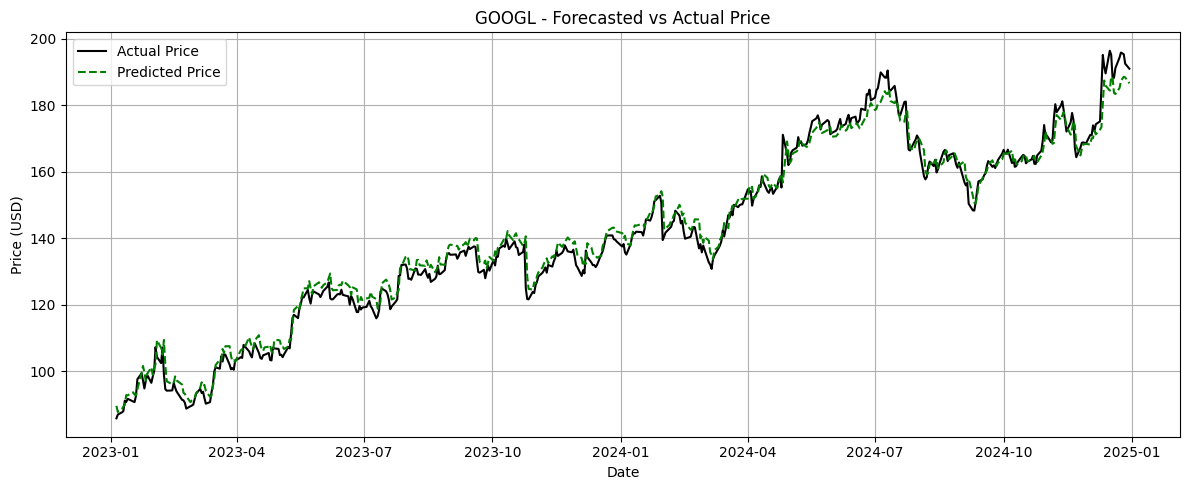
\includegraphics[trim=0cm 0cm 0cm 0.75cm,clip,width=0.8\linewidth]{images/GOOGL GRU quantum best.png}
    \caption{Predicted versus true prices for GOOGL using the hybrid quantum-classical model.}
    \label{fig:Google predictions hybrid}
\end{figure}

The model's predictions closely track the true stock price, often overestimating during upward trends and underestimating before price declines; patterns that could help identify potential buying and selling opportunities for traders. To assess the added value of the quantum layer, the same model was evaluated with the quantum layer disabled, which achieved a \textbf{Test MAE = 3.0522}, \textbf{Test RMSE = 3.9727}, and an \textbf{Average Absolute Percentage Error of 1.98\%}. Histograms showing the distribution of prediction errors for the classical model can be found in Appendix~\ref{appendix:classical error-hists}.



While the hybrid model shows a \textbf{slight improvement} over the classical baseline, the margin falls within typical predictive uncertainty ranges. As such, \textbf{no definitive advantage} of the quantum-enhanced model can be claimed based on this result alone. Further testing across additional datasets and scenarios would be required to conclusively demonstrate consistent performance gains from the hybrid approach.


\section*{4. Future Work}

While the hybrid quantum-classical model demonstrated promising results, several avenues remain for future improvement. One major limitation was the long runtime required to train and evaluate quantum layers. Implementing parallel processing, utilizing GPU acceleration, or deploying models on cloud-based quantum platforms could significantly speed up experimentation and allow for more consistent and thorough parameter sweeps without manual cross-referencing using the classical model. Further optimization could target additional hyperparameters such as the learning rate and explore alternative quantum circuit designs. The dataset itself could also be expanded to include more features or additional stock tickers, increasing generalization and robustness. Additionally, testing the quantum circuit on different platforms such as Qiskit or running on real quantum hardware offered by various providers could offer insight into platform-specific advantages or limitations. Finally, evaluating the model on live financial data or unseen stocks would help assess its real-world usability and performance beyond the original dataset.

\newpage
\appendix
\section{Appendix}
\subsection{Model Architecture Visualization}
\label{appendix:model-architecture}

\begin{figure}[H]
    \centering
    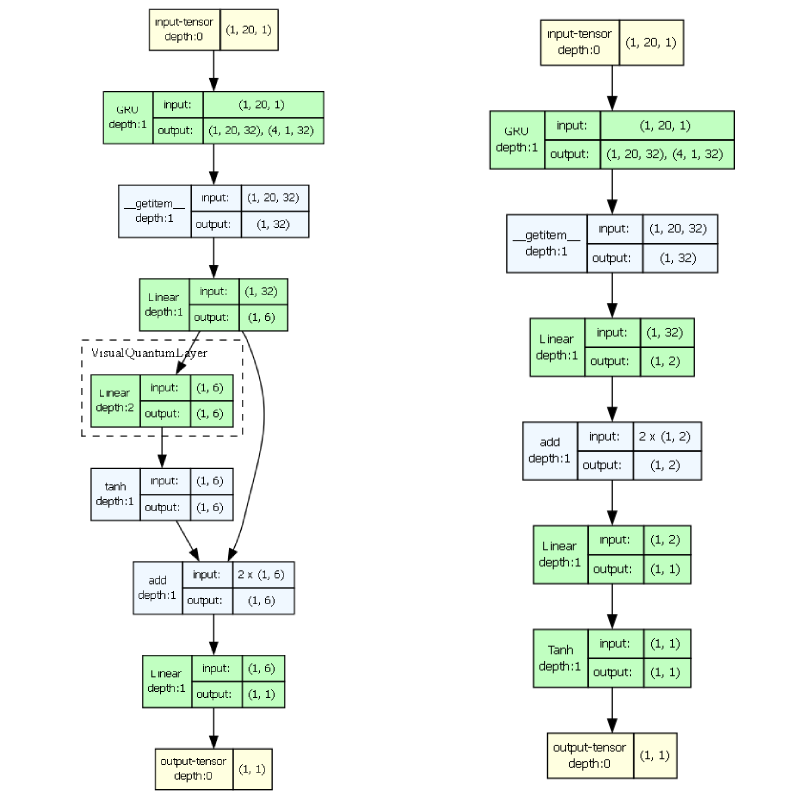
\includegraphics[trim=0cm 0cm 0cm 0cm, clip, width=0.85\linewidth]{images/model architecture.png}
    \caption{Model architecture overview. Left: Hybrid quantum-classical configuration. Right: Classical GRU-only baseline.}
    \label{fig:classical-vs-quantum}
\end{figure}

\subsection{Rotational Parameter Sweep Results}
\label{appendix:rotational-sweep}

\begin{figure}[H]
    \centering
    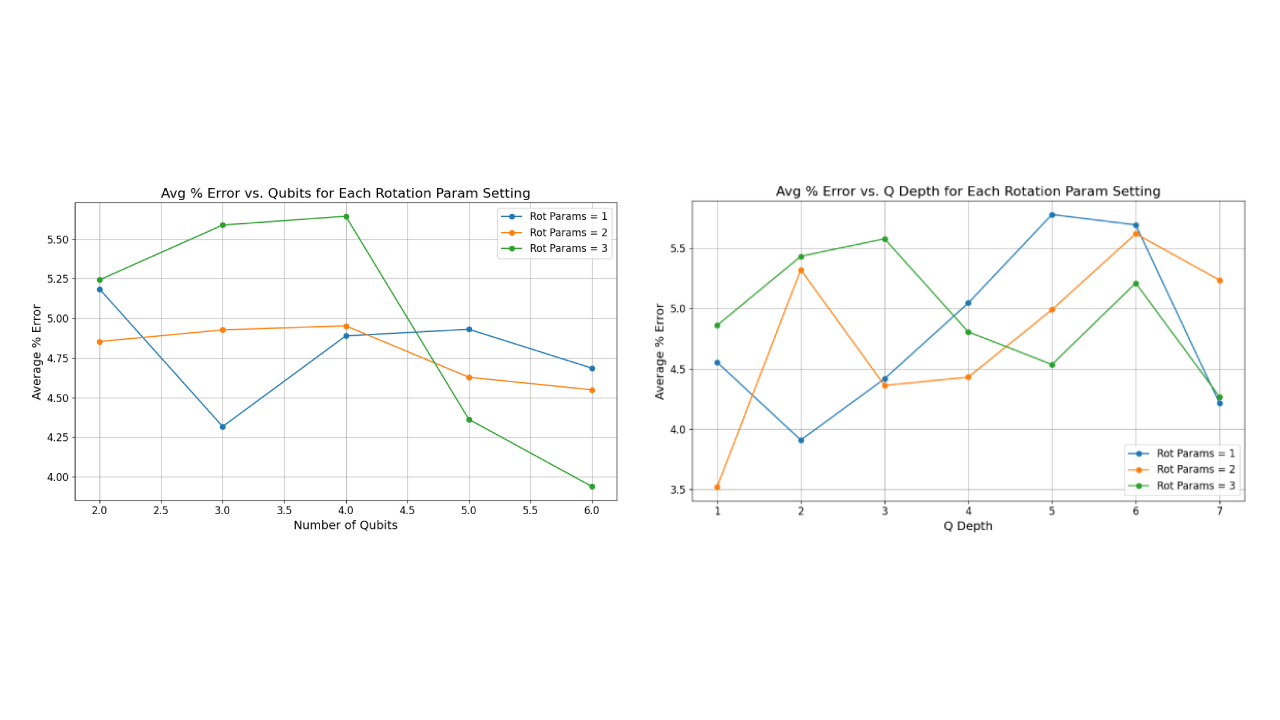
\includegraphics[trim=0cm 6cm 0cm 6cm,clip,width=1\linewidth]{images/quantum rotations.png}
    \caption{Average error segmented by rotation complexity across different qubit counts and depths.}
\end{figure}

\subsection{Classical Model Prediction Error Distributions}
\label{appendix:classical error-hists}

\begin{figure}[H]
    \centering
    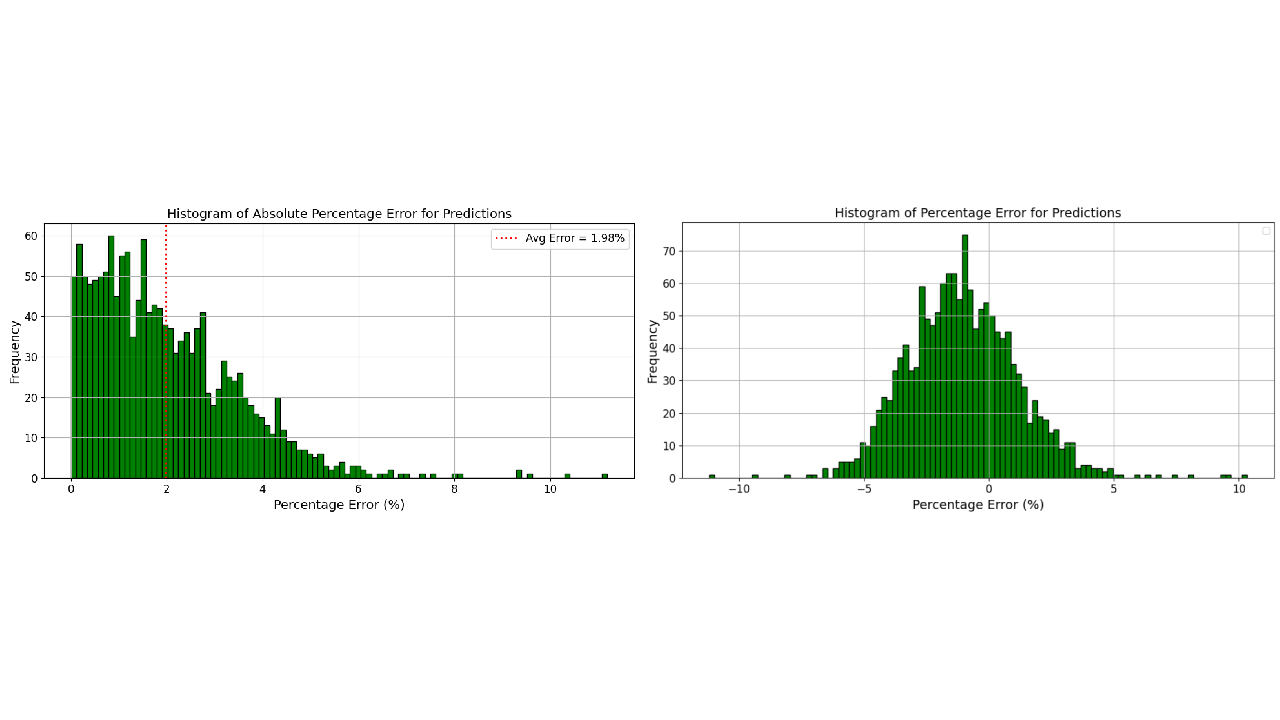
\includegraphics[trim=0cm 6cm -6cm 6cm,clip,width=1\paperwidth]{images/classical error hists.png}
    \caption{Distribution of prediction errors for the classical model.}
\end{figure}


\newpage
\bibliographystyle{ieeetr}
\bibliography{references}
\end{document}
